\documentclass{report}

\usepackage[margin=3cm]{geometry}
\usepackage{graphicx}
% \usepackage{subfigure}
\usepackage{caption} 
\captionsetup[table]{skip=0pt}
\usepackage{subcaption}
\usepackage{url}
\usepackage{hhline}

\usepackage{algorithm}
\usepackage{amsmath}
\DeclareMathOperator*{\argmin}{arg\,min}


\title{Random Walks course project\\Simulated Annealing Algorithm for Graph Coloring}

\author{
  R\'oger Berm\'udez Chac\'on\\EPFL
  \and
  Victor Kristof\\EPFL
  \and
  Merlin Nimier-David\\EPFL
}

\begin{document}
  \maketitle

  \paragraph{Abstract}
  We formulate the graph coloring problem as an optimization problem and use the Monte Carlo Markov Chain method to find proper colorings. Simulated annealing is used to improve the convergence speed. In this report, we recall the problem statement and formulation, present the simulated annealing schemes devised, give relevant implementation details and finally present results.

  % -----------------------------------------------------------------------------------
  \section*{Problem statement}
  \paragraph{Proper $q$-colorings}
  Let $G = (V, E)$ a graph with $|V| = N$. A \emph{coloring} using $q$ colors is an assignment $x \in \{ 1, \ldots, q \}^N$. A \emph{proper} $q$-coloring is a coloring such that no two adjacent edges have the same color: $(v, v') \in E \Rightarrow x_v \neq x_{v'}$. From this definition, we can define a cost function (Hamiltonian) to evaluate the ``quality'' of a given coloring:
  \[
    H(x) = \sum_{(v, v') \in E} 1_{x_v = x_{v'}}
  \]

  In the general case, finding the proper $q$-coloring of a graph of size $N$ is NP complete\footnote{\url{https://en.wikipedia.org/wiki/Graph_coloring#Computational_complexity}}, assuming $2 < q < N$. The search space is the domain of all colorings $x$, which has a size exponential in $N$. It is therefore interesting to relax the problem into an optimization problem. Using the cost function defined above:
  \[
    x^* = \argmin_{x \in \{ 1, \ldots, q \}^N} H(x)
  \]
  $x^*$ is a proper coloring when the minimum cost achieved is $0$. In the following section, we will describe how the Metropolis-Hastings algorithm can be used in this setting.

  \paragraph{Input data}
  In this project, we use Erd\"{o}s-R\'{e}nyi random graphs to test the correctness of our implementation and convergence speeds. They are constructed as follows: for a given density parameter $c$, each pair of the $N$ vertices is connected with probability $c / N$. Examples are given in Figure~\ref{Fig:random-graph-examples}, where an initial random coloring is also visualized.

  \begin{figure}[h]
      \centering
      \begin{subfigure}[t]{4.5cm}
        \centering
        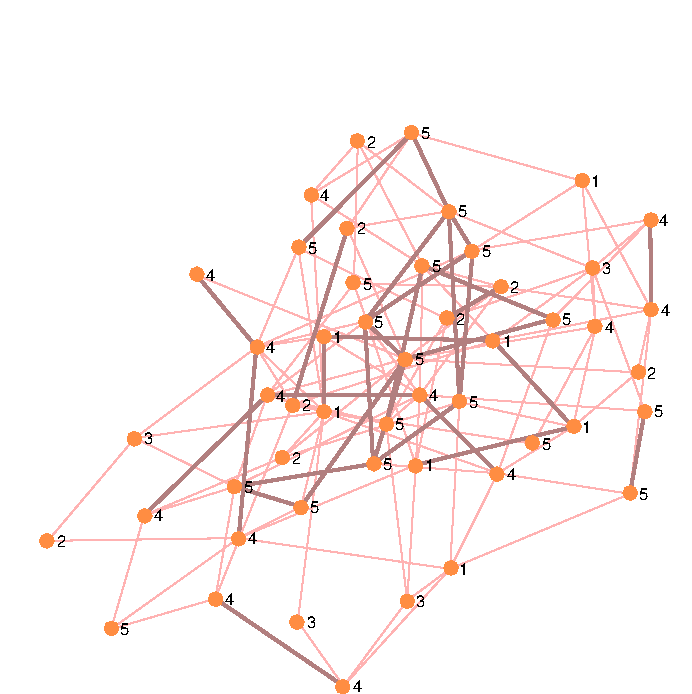
\includegraphics[width=4.5cm]{figures/random-graph-50-5-5.pdf}
        \caption{$c = 5$}
      \end{subfigure}
      \quad
      \begin{subfigure}[t]{4.5cm}
        \centering
        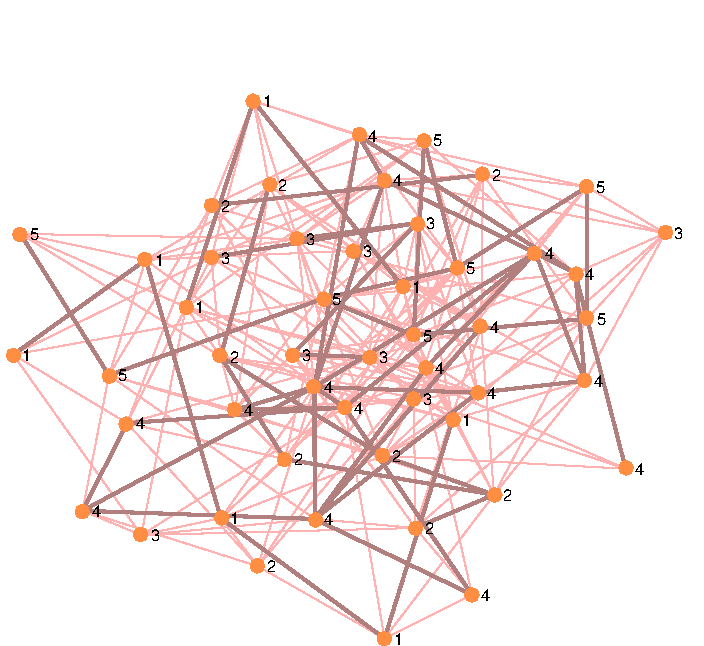
\includegraphics[width=4.5cm]{figures/random-graph-50-10-5.pdf}
        \caption{$c = 10$}
      \end{subfigure}
      \quad
      \begin{subfigure}[t]{4.5cm}
        \centering
        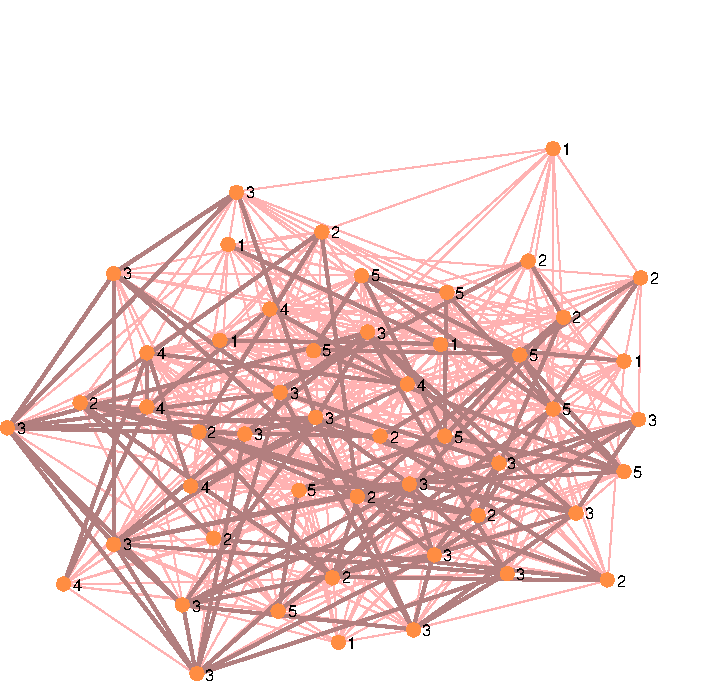
\includegraphics[width=4.5cm]{figures/random-graph-50-20-5.pdf}
        \caption{$c = 20$}
      \end{subfigure}

    \caption{Examples of Erd\"{o}s-R\'{e}nyi random graphs ($N = 50$ vertices) for different values of the density parameter $c$. We also visualize an initial random coloring: edges in bold represent a conflict between two vertices.}\label{Fig:random-graph-examples}
  \end{figure}

  % -----------------------------------------------------------------------------------
  \section*{MCMC solution}
  \paragraph{TODO} Describe how the optimization can be solved using Metropolis. Explain why we're convinced it will converge if there is a proper coloring.

  \paragraph{Simulated annealing}
  In order to find the global minimum of our cost function $H(x)$ that potentially contains several local minima, we make use of the \textit{simulated annealing}. This method simulates the physical process of cooling a solid such that when its structure is frozen, the minimum energy is reached. During the cooling procedure, we reduce the ``temperature'' $T$ or, equivalently, increase the ``inverse temperature'' $\beta=\frac{1}{T}$. The way the temperature is reduced is managed by a ``schedule'', a function of the current time step. In our implementation, we perform simulated annealing by increasing $\beta$ and the schedule will be referred to as $\beta(t)$.

  % -----------------------------------------------------------------------------------
  \section*{Results}
  \paragraph{Implementation details}
  TODO: Efficient implementations for generating the graph, transitioning, etc. Give some number to describe algorithm's performance (e.g. average time / iteration). Point out what can be parallelized (several independent chains with different initializations can run in parallel) and what cannot (a single chain).

  \paragraph{Experiments}  
  We define in Table \ref{tab:schedules} five different schedules, each depending on some parameters that must be tuned. The adaptive schedule is similar to the exponential one, except that $\alpha$ is now a function of $t$ (for instance, $\alpha(t) = 1/t$). For each schedules, $t$ can be replaced by $t-\tau$ in order to keep the inverse temperature constant for a while before starting to increase it. In this case, we have $\beta_{\tau}(t)=\max\left(\beta_0, \beta(t-\tau)\right)$.
  
  TODO: Give specific numbers for each parameter (min / max temperature used, starting point, etc). Show results plot for each. Pick the best one and give intuition as to why it performs better than the others.
  
  \begin{table}[h]
    \begin{center}
    \def\arraystretch{1.5}
      \begin{tabular}{|c||c|c|c|c|c|}
      	\hline
        \textbf{Schedules} & \textbf{Linear} &\textbf{Polynomial}  & \textbf{Logarithmic}& \textbf{Exponential} & \textbf{Adaptive} \\
        \hhline{|=||=|=|=|=|=|}
        \textbf{$\beta(t)$} & $\beta_0 + \alpha t$ & $\beta_0 t^{\alpha}$ & $\beta_0 \log (t + \alpha)$, $\alpha > 1$ & $\beta_0\alpha^{-t}$, $0 < \alpha < 1$ & $\beta_0\alpha(t)^t$ \\
      	\hline
	\textbf{Parameters} & \begin{tabular}[t]{@{}c@{}}$\beta_0=$ \\ $\alpha=$\end{tabular} &  \begin{tabular}[t]{@{}c@{}}$\beta_0=$ \\ $\alpha=$\end{tabular} &  \begin{tabular}[t]{@{}c@{}}$\beta_0=$ \\ $\alpha=$\end{tabular} &  \begin{tabular}[t]{@{}c@{}}$\beta_0=$ \\ $\alpha=$\end{tabular} &  \begin{tabular}[t]{@{}c@{}}$\beta_0=$ \\ $\alpha=$\end{tabular} \\
	\hline
      \end{tabular}
    \end{center}
    \caption{Schedules for $\beta$. Each of these equations gives $\beta(t)$, the value of $\beta$ at time step $t$.}
    \label{tab:schedules}
  \end{table}


  \begin{figure}
    \begin{center}
      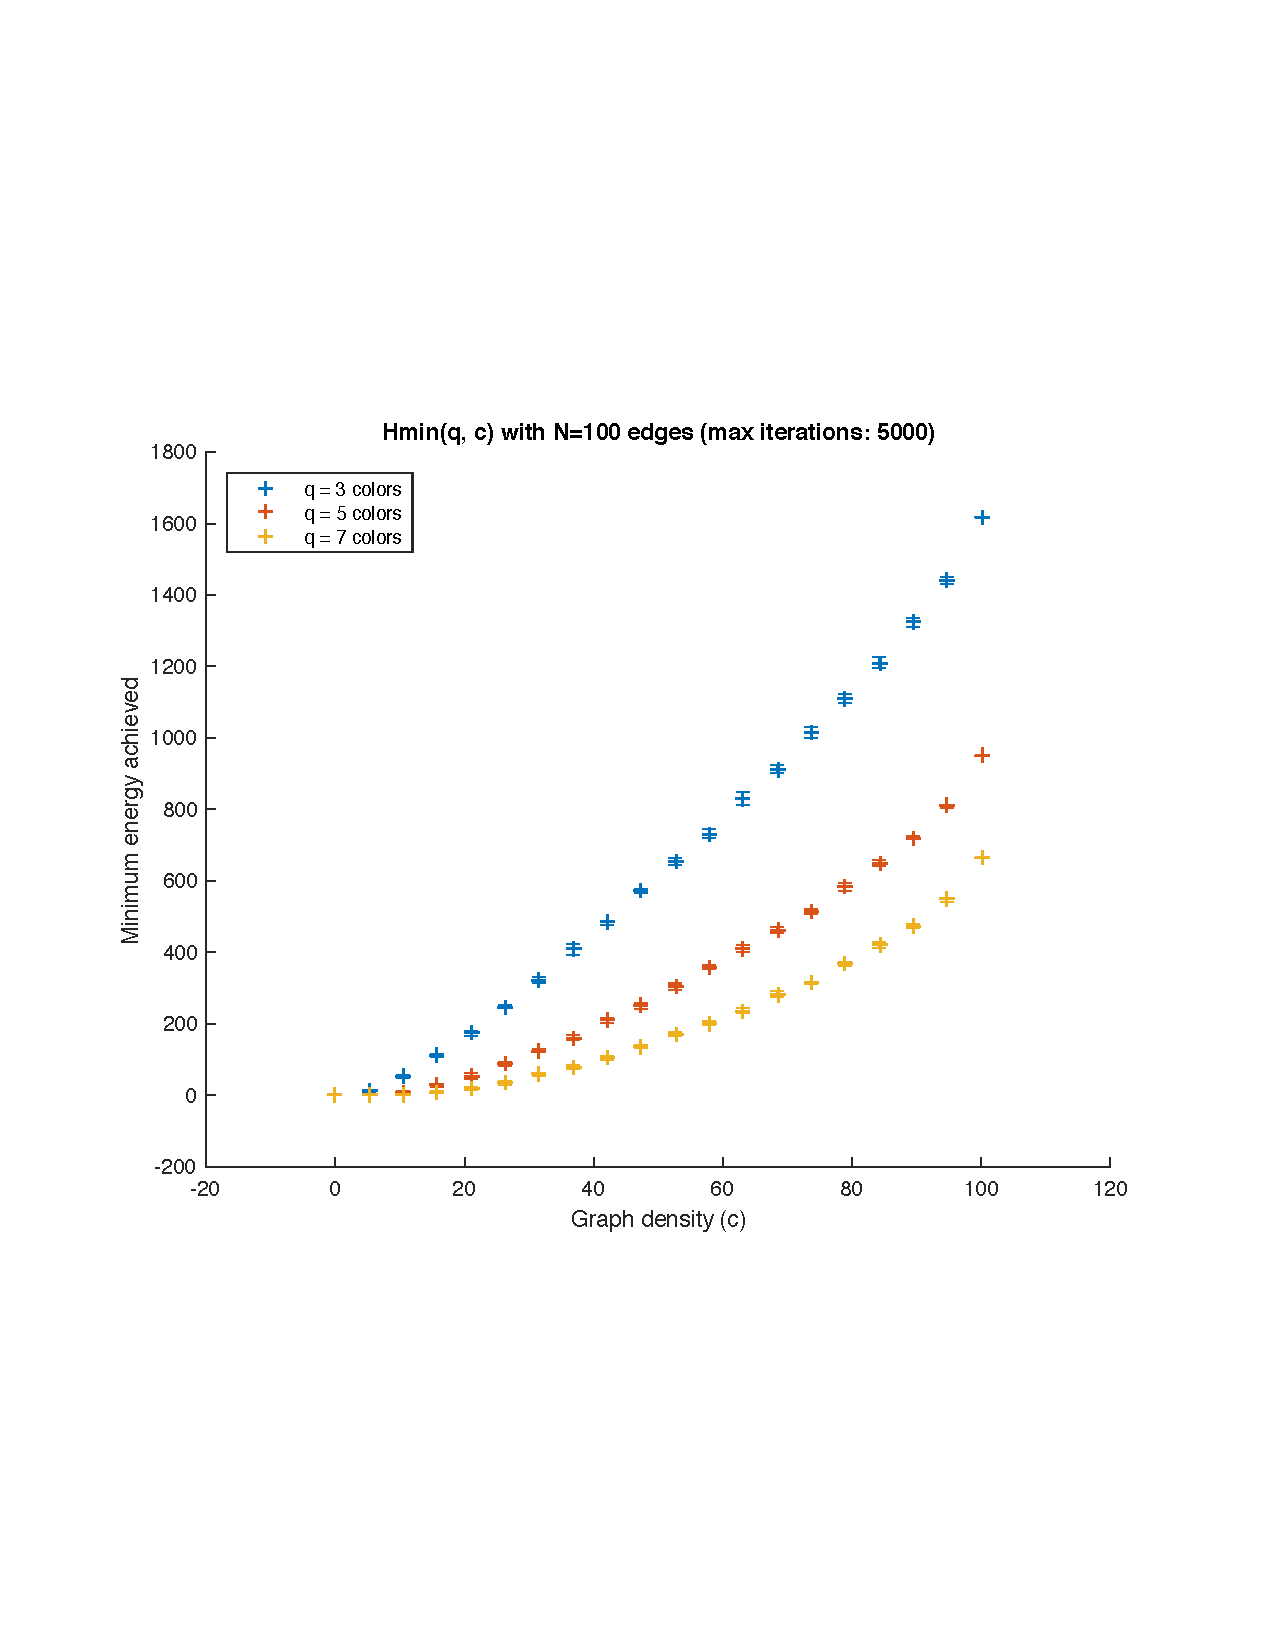
\includegraphics[width=8cm]{figures/cost-vs-graph-density.pdf}
    \end{center}
    \label{Fig:cost-vs-density}
    \caption{Minimal energy achieved as a function of graph density $c$ for different values of $q$. Since both the input data and the process are random, we perform the optimization for $5$ random inputs for each set of parameters and show error bars.}
  \end{figure}

\end{document}

